\subsection{Mächtigkeit von Mengen}
Für endliche (abzählbare) Mengen ist die Mächtigkeit gleichzusetzen mit der Anzahl
der Elemente einer Menge. Für unendliche (nicht abzählbare) Mengen müssen andere
Definitionen getroffen werden, um deren Mächtigkeit zu beschreiben.
\paragraph{Man schreibt:}
\({}|{}A{}|{}\) oder \(\#A\)
\paragraph{Es gilt:}
\begin{math}
{}|{}2^A{}|{} = 2^{{}|{}A{}|{}}
\end{math}
\subsubsection*{Gleichmächtigkeit}
Seien A und B zwei beliebige Mengen.
Dann heißt A gleichmächtig zur Menge B, wenn eine Bijektion (\({f:A}\rightarrow{B}\)) gebildet
werden kann. Das bedeutet, dass eine Vorschrift existiert, welches
jedem Element der Menge A genau ein Element der Menge B zuordnet.
Dabei werden alle Elemente der Menge B einmal erfasst. Diese
Vorschrift ist umkehrbar.
\paragraph{Man schreibt:} \(\#A = \#B\) bzw. \(|A| = |B|\)
\paragraph*{Beispiele:}
\begin{math}
\#{\mathbb N} = \#{\mathbb Z} = \#{\mathbb Q}
\end{math}
\subparagraph{Erläuterung zu \(\#{\mathbb N} = \#{\mathbb Z}\):} Der
Einwand, dass die natürlichen Zahlen doch 'offensichtlich' (von der 0
abgesehen) doppelt so viele seien müssten, wie die ganzen Zahlen zählt
bei diesen unendlichen Mengen nicht! Stattdessen sollte man an die
Definition der Gleichmächtigkeit denken: 2 Mengen sind dann gleich,
wenn man eine eineindeutige(bijektive) Abbildung finden kann.
\begin{figure}[b]
  \centering
  \caption{Beispiel für eine Abbildung \(\#{\mathbb N} = \#{\mathbb Z}\)}
  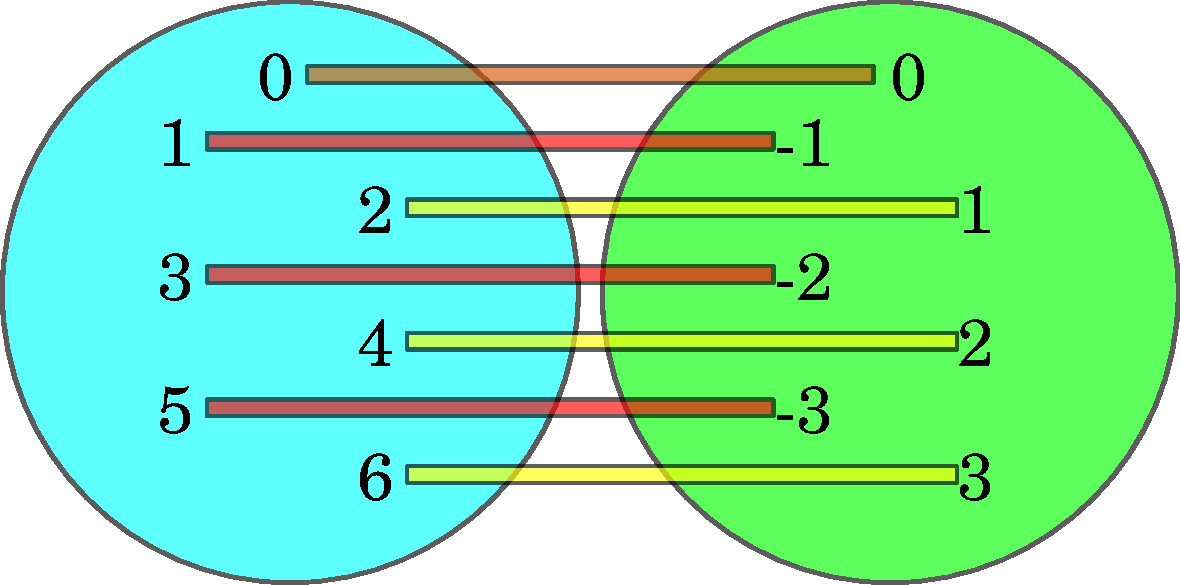
\includegraphics[scale=0.5]{ngleichz.pdf}
\end{figure}
Es werden also die 0 auf die 0, die ungeraden Zahlen auf die positiven
Zahlen und die geraden Zahlen auf die negativen Zahlen abgebildet.
Dies ist aufgrund der Unendlichkeit der beiden Mengen ohne Probleme
möglich.

Auch für die rationalen Zahlen lässt sich ein solches Schema für eine Bijektion finden.
Hierauf geht ein Wikipedia-Artikel näher ein:

% J.S.: Wir sollten die Wikipedia-Artikel später in das Skript einarbeiten..
\url{http://de.wikipedia.org/wiki/Cantors_erstes_Diagonalargument}

Und auch bei der Frage, warum die reellen Zahlen nicht abzählbar sind, hilft Wikipedia:

\url{http://de.wikipedia.org/wiki/Cantors_zweites_Diagonalargument}
